\section{Przypadek Testowy 5 - Algorytm genetyczny - zależność PRD od wybranej metody krzyżowania}
  \subsection{Cel:}
    Celem tego testu będzie sprawdzenie, w jakim stopniu otrzymywane wyniki zależą od wybranej metody krzyżowania. W naszej implementacji
    algorytmu genetycznego znalazły się dwie metody krzyżowania:
    \begin{itemize}
      \item Partially Mapped Crossover (PMX)
      \item Cycle Crossover (CX)
    \end{itemize}
    Testy wykonano na wybranych instancjach z biblioteki TSPLIB:
    \begin{enumerate}
      \item gr48.tsp
      \item gr21.tsp
      \item berlin52.tsp
      \item gr120.tsp
      \item br17.atsp
      \item ftv47.atsp
      \item ftv70.atsp
      \item kro124p.atsp 
    \end{enumerate}
    Wszystkie parametry wywołania pozostały niezmienne przez cały okres wykonywania testów.
  \subsection{Wyniki: }
  \textbf{UWAGA}: W poniższej tabeli kolumna \textit{Różnica} oznacza różnicę między otrzymanymi średnimi wartościami PRD dla testowanych metod krzyżowania.
  Dodatnia wartość różnicy świadczy o tym, iż w danym teście lepsze wyniki średnio produkowały wywołania wykorzystujące metodę krzyżowania CX, natomiast 
  ujemna różnica świadczy o lepszych wynikach metody PMX. \\
    Poniższa tabela przedstawia uśrednione wyniki testów:
    \begin{table}[!ht]
      \centering
      \begin{tabular}{| c | c | c | c |}
        \hline
        Instancja & PMX & CX & Różnica \\
        \hline
        gr48.tsp & 3.324 \%& 3.506 \% & -0,182 \%\\
        gr21.tsp & 3.746 \%& 3.502 \%& 0,244 \%\\
        berlin52.tsp & 8,096 \%& 7,362 \% & 0,734 \%\\
        br17.atsp & 0 \%& 0 \%& 0 \%\\
        ftv47.atsp & 39,3 \%& 35,8 \%& 3,5 \%\\
        ftv70.atsp & 25,898 \%& 32,482 \%& -6,584 \%\\
        kro124p.atsp & 27,184 \%& 26,008 \%& 1,176 \%\\

        \hline
          
      \end{tabular}
      \caption{Tabela zależności otrzymanych wyników PRD od wybranej metody krzyżowania}
    \end{table}
  \subsection{Wykresy: }
  \begin{figure}[H]
    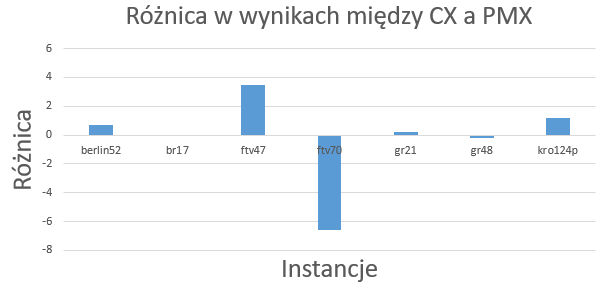
\includegraphics[scale=0.75]{krzyzowania.png}
    \centering
    \caption{Otrzymane różnice dla wskazanych metod krzyżowań}
  \end{figure}
  \subsection{Wnioski: }
    Z testów wynika, iż nie można jednoznacznie określić, która z metod krzyżowania osobników jest uniwersalnie lepsza, zauważamy, iż odpowiednie metody
    radzą sobie lepiej od pozostałych dla odpowiednich przykładów.